\documentclass{article}
\usepackage{color}
\usepackage{tikz}
\usepackage{float}
\usepackage{tabularx}
\usepackage{amsmath}
\usepackage{amssymb}
\usepackage{listings}
\usepackage{enumitem}
\usepackage{syntax}
\usepackage{csquotes}
\usepackage[backend=biber]{biblatex}
\addbibresource{references.bib}

\usepackage{tikz}
\usetikzlibrary{automata,positioning}

\definecolor{dkgreen}{rgb}{0,0.6,0}
\definecolor{gray}{rgb}{0.5,0.5,0.5}
\definecolor{mauve}{rgb}{0.58,0,0.82}


\lstset{frame=tb,
  numbers=left,
  stepnumber=1,
  language=Java,
  aboveskip=3mm,
  belowskip=3mm,
  showstringspaces=false,
  columns=flexible,
  basicstyle={\small\ttfamily},
  numberstyle=\color{gray},
  keywordstyle=\color{blue},
  commentstyle=\color{dkgreen},
  stringstyle=\color{mauve},
  breaklines=true,
  breakatwhitespace=true,
  tabsize=2,
  moredelim=**[is][\color{red}]{@}{@},
}

\setlength{\grammarindent}{12em}

%\renewcommand{\lstlistingname}{Algorithm}
%\newcommand{\tablerow}[4]{ #1 & #2 & #3 & #4\\}
\newcommand{\n}[0]{\\[\baselineskip]}
%\newcommand{\qa}[2]{\textbf{Q:} #1 \\ \textbf{A:} #2}
%\newcommand{\argument}[4]{\textbf{#1:} #2 \\ \textbf{#3:} #4}

\title{CS4303 Geometry Wars Report}
\author{140011146}

\begin{document}

\maketitle

\section{Introduction}
In this practical we were tasked to implement a top-down shooter game, similar to games like \textit{Robotron 2084} and \textit{Geometry Wars} with the goal of implementing a variety of AI algorithms. In my game, I have implemented six different types of AI, including a flocking AI. I have also implemented multiple different pickups and the ability to play over a network.
\n
To build the game, run \texttt{ant} in the submission directory.
\\
\noindent
To run the server, run \texttt{ant -Darg0="Server" server}
\\
\noindent
To run the client, run \texttt{ant -Darg0="Name" client} where ``Name" can be any name.
\section{Game features and design}
\subsection{AI Enemies}
\subsubsection{Basic chase}
\begin{figure} [H]
\centering

\includegraphics[width=0.1\textwidth, keepaspectratio]{imgs/BasicChaseEnemy.png}
\caption{Basic Chase Enemy}
\end{figure}
\noindent
This is the most basic AI that always goes towards the current position of the player. If the player is always moving, this AI will always be chasing behind the player, making it quite easy to run away from.

\subsubsection{Circle}
\begin{figure}[H]
\centering

\includegraphics[width=0.1\textwidth, keepaspectratio]{imgs/CircleEnemy.png}
\caption{Circle Enemy}
\end{figure}
\noindent
This AI is similar to the basic chase AI except they use acceleration in their movement rather than moving at a constant speed towards the player's position. This means that if the player moves past the quickly, they will take more time to reverse and follow the player again. 

\subsubsection{Ambush}
\begin{figure}[H]
\centering

\includegraphics[width=0.1\textwidth, keepaspectratio]{imgs/AmbushEnemy.png}
\caption{Ambush Enemy}
\end{figure}
\noindent
This AI attempts to move towards where it predicts the player will be based on the direction the player is moving in. It will move to a position in front of the player. 
\n
I found when first creating this AI that if it implements this behaviour and there are a lot of them, they will all move synchronously when the player changes direction, making them easy to predict for a player. To deal with this, I added a random delay before they change their target position making each of them act more independent.

\subsubsection{Patrol}
\begin{figure}[H]
\centering

\includegraphics[width=0.1\textwidth, keepaspectratio]{imgs/PatrolEnemy.png}
\caption{Patrol Enemy}
\end{figure}
\noindent
These AI spawn in with the generated pickups and will patrol in a square around the pickups. If the player comes near they will chase the player for a certain distance before moving back to their patrol locations. 

\subsubsection{Shoot}
\begin{figure}[H]
\centering

\includegraphics[width=0.1\textwidth, keepaspectratio]{imgs/ShootEnemy.png}
\caption{Shooting Enemy}
\end{figure}
\noindent
This AI will shoot back at the player, making it more difficult. I chose to make them shoot directly at the player position rather than randomly near the player so it is easier to dodge if the player is always moving. These AI will move randomly around the screen while shooting.

\subsubsection{Flocking}
\begin{figure}[H]
\centering
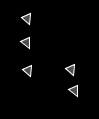
\includegraphics[width=0.1\textwidth, keepaspectratio]{imgs/FlockingEnemy.png}
\caption{Flocking Enemy}
\end{figure}
\noindent
The flocking algorithm was implemented following the example on https://processing.org/examples/flocking.html \cite{flocking}. 
\n
Initially these enemies moved towards the player position if there were no nearby flockmates but this made the game very hard as they would all flock towards the player. Instead, their initial target position is the player's current position and there is no other target direction or velocity when there are no nearby flockmates. 
\n
These AI are also smaller and more are spawned in the game to show off their flocking behaviour without filling the whole screen.

\subsection{AI Director}
\subsubsection{Pacing}
The AI director uses an adaptive pacing algorithm following the system used in Left 4 Dead \cite{l4d}. The idea is to have bouts of high intensity and low intensity, the durations of which change dynamically. The ``intensity" of players is roughly estimated:
\begin{itemize}
\item Increase intensity when the player takes damage, proportional to the damage.
\item Increase intensity when the player kills an enemy, proportional to the score value of killed enemy.
\item Decrease intensity over time. 
\end{itemize}
\noindent
If the intensity is too high, no shooting enemies are spawned to make the game a little easier for the players.

\begin{figure}[H]
\centering
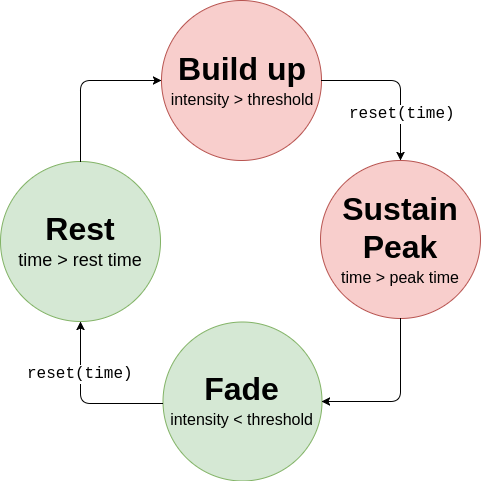
\includegraphics[width=0.7\textwidth, keepaspectratio]{imgs/DirectorFSM.png}
\caption{State machine of the AI director.}
\end{figure}
\noindent
The \textbf{Build up} and \textbf{Sustain Peak} states have a higher spawn rate of enemies. The director moves from build up to sustain peak when the intensity is greater than the threshold. The sustain peak state is there to ensure there is some minimum time spent with high spawn rates of enemies. 
\n
\textbf{Fade} and \textbf{Rest} states are the opposite side to build up and peak. The director moves out of fade when the intensity is below the threshold and rest acts the same as peak, ensuring a minimum period of rest before the next build up.
\subsubsection{Difficulty}
At regular intervals, the state of the game is sampled to see how well the players are doing and adjust the difficulty accordingly. By default, the difficulty slowly increases at each interval to progressively make the game harder.
\n
An increase in the difficulty value of the game affects the following parameters:
\begin{itemize}
\item Increased enemy health
\item Increased enemy damage to players
\item Increased enemy score value
\item Increased enemy spawn rate
\item Decreased pickup spawn rate
\item Decreased pickup lifespan
\end{itemize}

\subsection{Weapons}
The player is equipped with three different weapons that can be quickly swapped at any point. Each weapon has a separate ammo and reload system, making it convenient if the player runs out of ammunition on one weapon to switch to another rather than wait for the reload.
\subsubsection{Pistol}
\begin{figure}[H]
\centering

\includegraphics[width=0.1\textwidth, keepaspectratio]{imgs/Gun.png}
\caption{Player with pistol equipped}
\end{figure}
\noindent
The pistol is a simple weapon with low clip size and low fire rate and faster reload.

\subsubsection{Rocket}
\begin{figure}[H]
\centering

\includegraphics[width=0.1\textwidth, keepaspectratio]{imgs/Rocket.png}
\caption{Player with rocket equipped}
\end{figure}
\noindent
The rocket is a powerful weapon that creates an explosion on impact, dealing lots of damage but it comes with extremely low clip size, low fire rate and slow reload.

\subsubsection{Machine gun}
\begin{figure}[H]
\centering

\includegraphics[width=0.1\textwidth, keepaspectratio]{imgs/MachineGun.png}
\caption{Player with machine gun equipped}
\end{figure}
\noindent
The machine gun shoots bullets quickly with a larger clip size and high fire rate but takes longer to reload.


\subsection{Pickups}
\subsubsection{Health pickup}
\begin{figure}[H]
\centering

\includegraphics[width=0.1\textwidth, keepaspectratio]{imgs/HealthPickup.png}
\caption{Health pickup}
\end{figure}
\noindent
The health pickup gives the player more health. A player is able to go over the maximum 100 health when picking up these pickups to act as a buffer for more health, but this will signal to the AI director that the player is doing well.
\subsubsection{Ammo pickup}
\begin{figure}[H]
\centering

\includegraphics[width=0.1\textwidth, keepaspectratio]{imgs/AmmoPickup.png}
\caption{Ammo pickup}
\end{figure}
\noindent
The ammo pickup increases the ammo of each of the player's weapon by one clip. It is important to pick up these, otherwise the players will eventually run out of ammunition.
\subsubsection{Speed pickup}
\begin{figure}[H]
\centering

\includegraphics[width=0.1\textwidth, keepaspectratio]{imgs/SpeedPickup.png}
\caption{Speed pickup}
\end{figure}
\noindent
This pickup temporarily increases the speed of the player who picked it up. This is useful to run away or reach a far pickup quickly, but it is a double-edged sword as the player can easily run head-on into a group of enemies.
\subsubsection{Pierce pickup}
\begin{figure}[H]
\centering

\includegraphics[width=0.1\textwidth, keepaspectratio]{imgs/PiercePickup.png}
\caption{Pierce pickup}
\end{figure}
\noindent
The pierce pickup will allow the player's bullets to pierce through all enemies. This does not apply to the rocket weapon.

\subsubsection{Damage pickup}
\begin{figure}[H]
\centering

\includegraphics[width=0.1\textwidth, keepaspectratio]{imgs/DamagePickup.png}
\caption{Damage pickup}
\end{figure}
\noindent
This pickup permanently increases the player's damage. This helps the player deal with the increased health of enemies from increasing difficulty.

\subsubsection{Bullet radius pickup}
\begin{figure}[H]
\centering

\includegraphics[width=0.1\textwidth, keepaspectratio]{imgs/RadiusPickup.png}
\caption{Bullet radius pickup}
\end{figure}
\noindent
This pickup permanently increases the player's bullet's radius. This helps the player with easily aim as the larger bullets will catch enemies easier, especially when trying to shoot the flocking enemies. This increased radius also affects the rocket's explosion size, as it scales off the rocket bullet's radius.

\subsubsection{Bomb pickup}
\begin{figure}[H]
\centering

\includegraphics[width=0.1\textwidth, keepaspectratio]{imgs/BombPickup.png}
\caption{Bomb pickup}
\end{figure}
\noindent
This is a powerful pickup that will clear the entire screen of enemies, giving players a brief respite. 

\subsection{Networking}

\section{Implementation details}


\subsection{Factories}

\subsection{Network}
To implement the networking in the game, I use a processing UDP library (https://ubaa.net/shared/processing/udp/).
\n
UDP packets are sent on every frame of the game. The server will send the entire game state and let the client render the state. Clients only send the player input to the server to process. This means the server is always correct and would prevent client players from cheating their attributes such as position and health. The trade off is the server has to do a lot more processing and so the game cannot scale to having many players at once.


\subsection{Pickups}

\section{Conclusion}


\printbibliography

\end{document}
